%LaTex的图片插入,缩放,旋转angle  %参照CTEX中文套装graphics.pdf
%eps图片生成方式
%1. 通过软件生产,如matlab
%2. 通过acrobat pro制作(适用于提取PDF中的图片)
%3. 借助WORD,PDF打印机和acrobat pro制作(适用于emf,wmf等格式)
%具体操作保存在为知笔记云端中

\documentclass{book}

\usepackage{mathrsfs}
\usepackage{amsmath}
\usepackage{graphicx} %插入图片的宏包

\numberwithin{equation}{section}  %使公式编号按照章节来编号

\begin{document}
\chapter{Intro}

%插入图片的命令:includegraphics
%includegraphics命令支持导入eps格式和点阵位图的图片
%eps格式文件可以用记事本打开
%eps格式由adobe公司发明,支持不失真操作

\includegraphics{cat.eps}
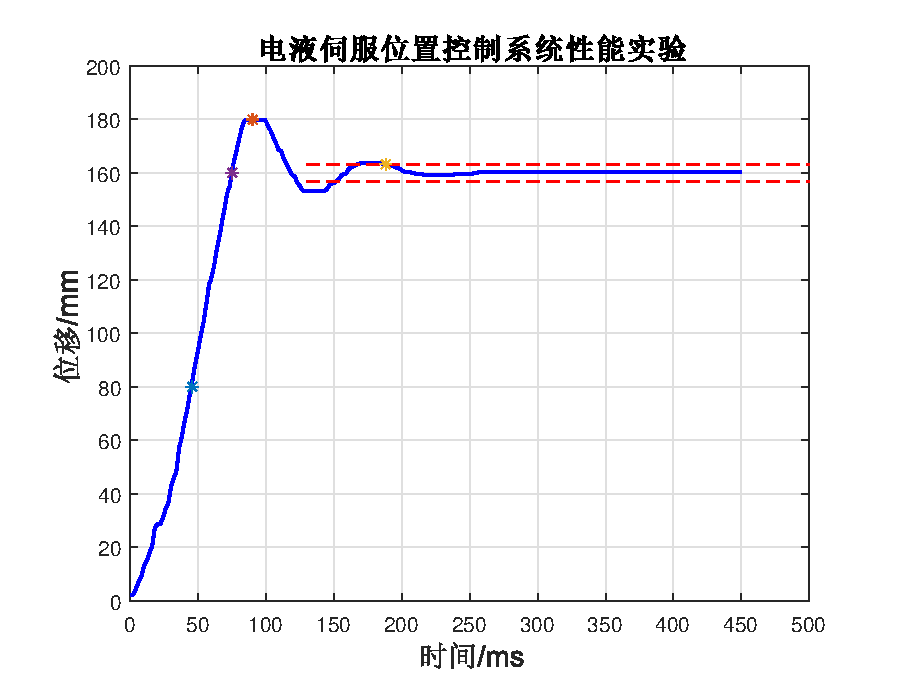
\includegraphics{valve.eps}

%图片操作环境figure
\begin{figure}
	\centering %图片居中
	%图片放大scale倍,旋转angle度
	
\includegraphics[scale=6,angle=30]{cat.eps} 
	\caption{This is a cat}
\end{figure}


\chapter{Intro1}
%利用图片向导创建
\begin{figure}
	\centering
	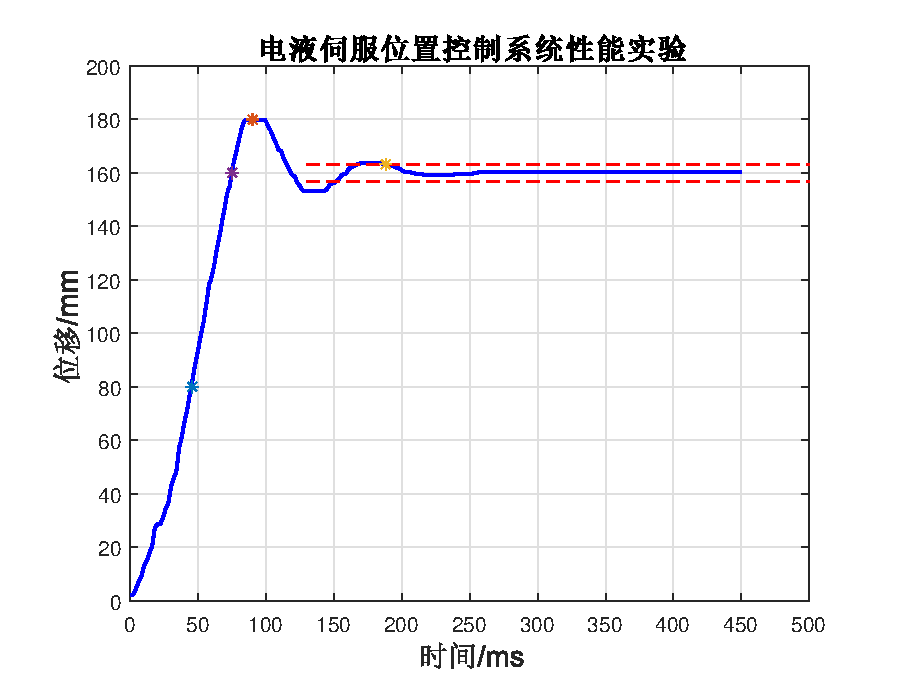
\includegraphics[width=0.7\linewidth]{valve}
	\caption[short]{This a figure generated by Matlab}
	\label{fig:valve}
\end{figure}

\chapter{Intro2}

\end{document}